\chapter{Adaptive Optik\label{chapter:thema}}
\lhead{Adaptive Optik}
\begin{refsection}
\chapterauthor{Matthias Schneider}

\section{Einleitung}
In diesem Kapitel wird das Thema \textit{Adaptive Optik AO} behandelt, dazu werde ich zuerst eine kurze Übersicht über das Thema geben und anschliessend einige Aspekte genauer erklären. Beim kürzesten Weg geht geht es darum zu zeigen, welchen Weg ein Lichtstrahl geht, wenn er von $A$ nach $B$ muss und auf dem Weg eine Phasengrenze ist. Bei Teleskopen mit adaptiver Optik wird mit Laser ein Leitstern erzeugt, welcher als kugelförmige Referenzlichtquelle dient, trotzdem rechnen wir mit ebenen Wellen. Im Abschnitt Wellenfront wird erklärt weshalb das möglich ist. Im letzten Abschnitt wird die Idee vom kürzesten Weg verallgemeinert, was dann zur Eikonalgleichung führt, mit welche dargestellt werden kann, wie sich die Wellenfronten verformen. 

\section{Adaptive Optik und ihre Anwendungen}
Adaptive Optik (AO) ist eine Technik, mit der optische Systeme verbessert werden können. Dabei können aber nur Fehler korrigiert werden, welche im Medium zwischen der Quelle des Lichtes und dem Sensor entstehen, hauptsächlich geht es also darum, Fehler, die durch die Atmosphärenunruhe entstehen zu kompensieren. Die erdgebundene Astronomie ist heute auf diese Technologie angewiesen, denn Beobachtungen im optischen und infraroten Bereich sind nur möglich, wenn die negativen Effekte der Atmosphäre korrigiert werden können. Ein Beispiel dazu ist die Abbildung \ref{fig:jupiter}, sie zeigt eine Aufnahme des Jupiters mit dem Very Large Telescope (VLT) der European Southern Observatory (ESO).
\begin{figure}
  \centering
  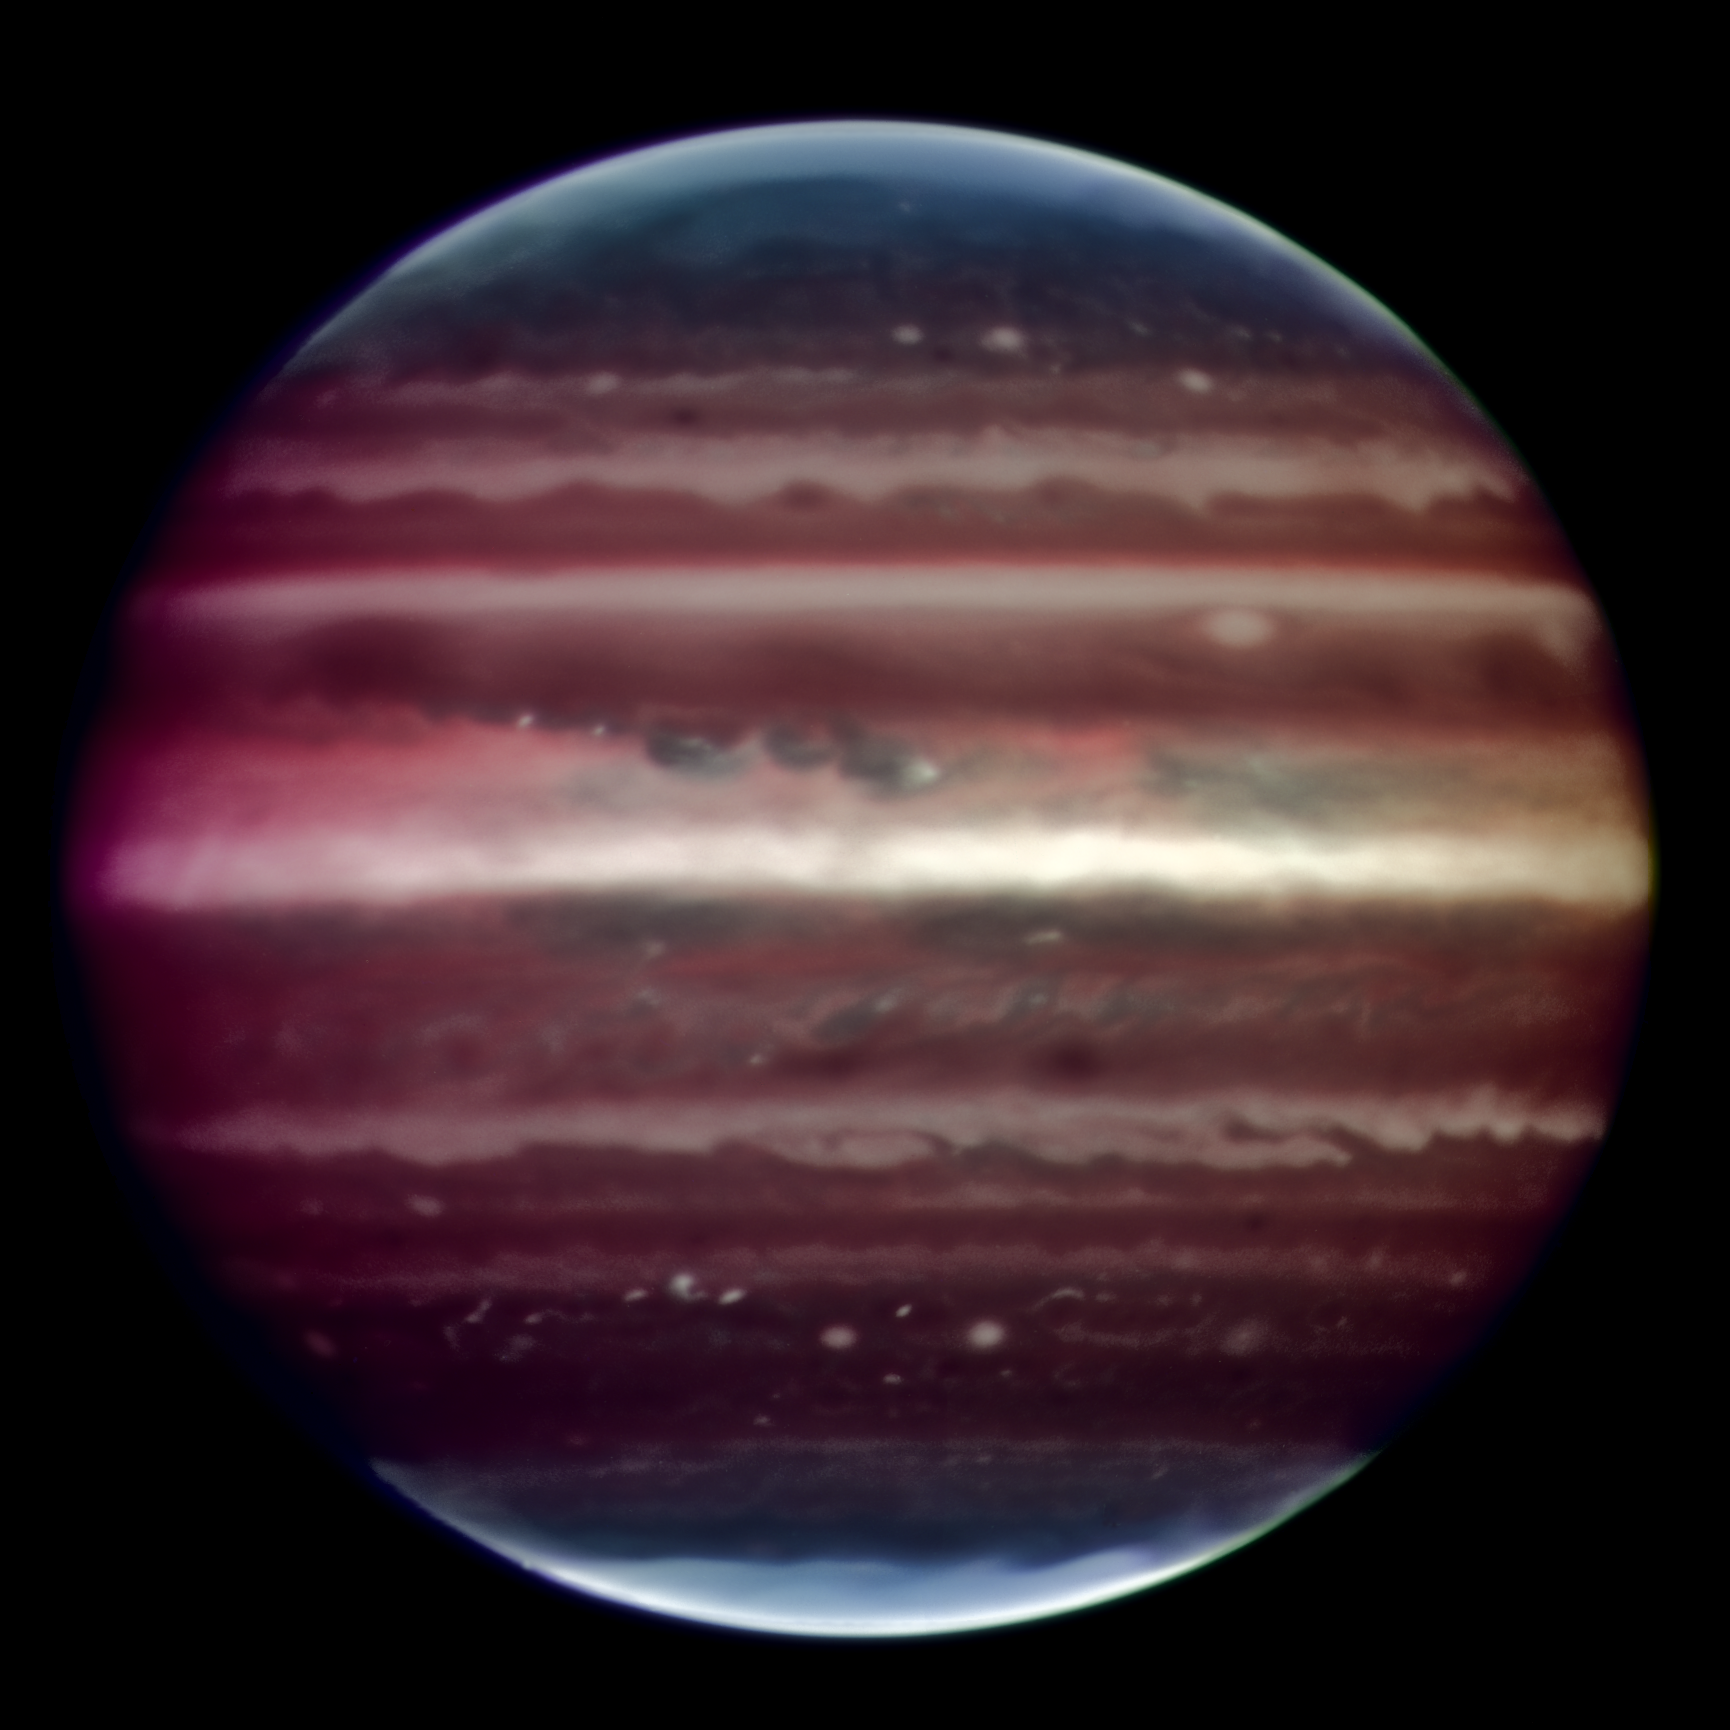
\includegraphics[width=0.6\textwidth]{adaptiv/images/Jupiter_adaptiv}
  \caption{Jupiter mit adaptiver Optik von der Erde aus mit VLT aufgenommen
    \cite{eso:jupiter}}
  \label{fig:jupiter}
\end{figure}

Adaptive Optik wird heute aber auch bei anderen Anwendungen eingesetzt, um die Präzision von optischen Apparaturen zu erhöhen, so gibt es beispielsweise Mikroskope mit AO. Ein weiterer Einsatzbereich dieser Technologie ist der Fokusiserspiegel von Laserschneidanlagen, womit eine deutliche Steigerung der Präzision beim Schneiden erreicht werden kann.

Ein System mit einer adaptiven Optik ist aus drei Hauptkomponenten aufgebaut. Ein Sensor misst die Störung der Wellenfront, einen Computer berechnet die benötigte Korrektur und mit einem beweglichen Spiegel kann die Wellenfront korrigiert werden. So ist es möglich, auf dem Messinstrument, welches das Nutzsignal misst, trotz nicht optimalen Bedingungen ein möglichst scharfes Bild zu haben.

Als Sensor wird für gewöhnlich eine Hartmannplatte verwendet, welche aus einem Mikrolinsenarray besteht und pro Linse einen CMOS oder CCD-Sensor hat. Mit diesem kann  die Verkippung der Wellenfront im Bereich einer einzelnen Linse bestimmt werden. Auf der Abbildung \ref{fig:hartmannplatte} ist gut zu erkennen, was geschieht, wenn die Wellenfront nicht mehr eben, sondern durch die Atmosphäre leicht gestört wird. Das Licht des Leitsterns wird durch die einzelnen Linsen des Arrays nicht mehr in die Mitte des Sensors fokussiert, sondern leicht verschoben. Diese Verschiebung wird gemessen und daraus die benötigte Korrektur berechnet, damit der bewegliche Spiegel in Stellung gebracht, und die Wellenfront nahezu ohne Störung in das Messinstrument geleitet. Dieser Zyklus aus Störung messen, Korrektur berechnen und Spiegel in Stellung bringen, wird etwas 1000 mal pro Sekunde wiederholt, was auch eine hohe Leistung und Spezialisierung des Korrekturrechners erfordert. Dazu wird oft eine Regelstrecke aufgebaut, mit welcher dieser Zyklus geregelt werden kann. Auf der Abbildung \ref{fig:schematischAO} ist dieser Regelkreis schematisch dargestellt.

\begin{figure}
  \centering
  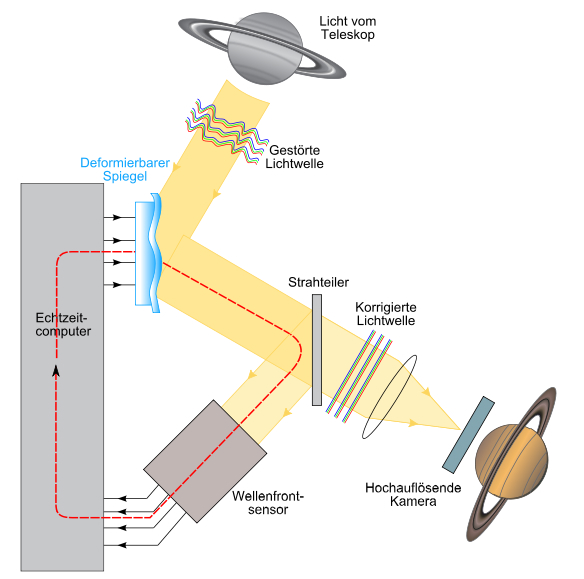
\includegraphics[width=0.9\textwidth]{adaptiv/images/schematichAO}
  \caption{Schematische Darstellung des Regelkreises einer AO
    \cite{robani:schematischAO}}
  \label{fig:schematischAO}
\end{figure}

\begin{figure}
  \centering
  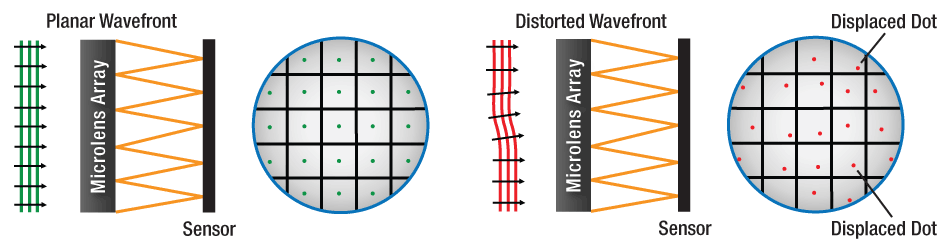
\includegraphics[width=0.95\textwidth]{adaptiv/images/hartmannplatte}
  \caption{Hartmannplatte mit ebener und verformter Wellenfront
    \cite{thor:hartmannplatte}}
  \label{fig:hartmannplatte}
\end{figure}

Ein weiteres wichtiges Element bei der adaptiven Optik ist das Erzeugen einer Referenzquelle, durch welche ein Signal entsteht, das bekannt ist und wodurch der Einfluss der Atmosphäre gemessen werden kann. In der Astronomie wird dazu mit Laser ein künstlicher Stern erzeugt, der sogenannte Leitstern. Er wird in einer Höhe von etwa 90$km$ erzeugt, also am oberen Ende der Mesosphäre. Dazu wird oft ein Natrium-Laser verwendet, der eine Wellenlänge von 589$nm$ hat. Damit wird die beim Natrium die D-Linie angeregt, was der Farbe der Strassenbeleuchtung entspricht. Das Licht des Natrium-Lasers wird von den Natriumatomen in der Höhe von 90$km$ zurückgeworfen. Dabei wird angenommen, dass dabei ein Stern entsteht, dessen Licht sich Kugelförmig ausbreitet. Wichtig ist dabei, dass der Stern in Beobachtungsrichtung des Teleskops erzeugt wird, damit nur die Atmosphäre, in welcher störende Einflüsse sind, gemessen wird. 


\begin{figure}
  \centering
  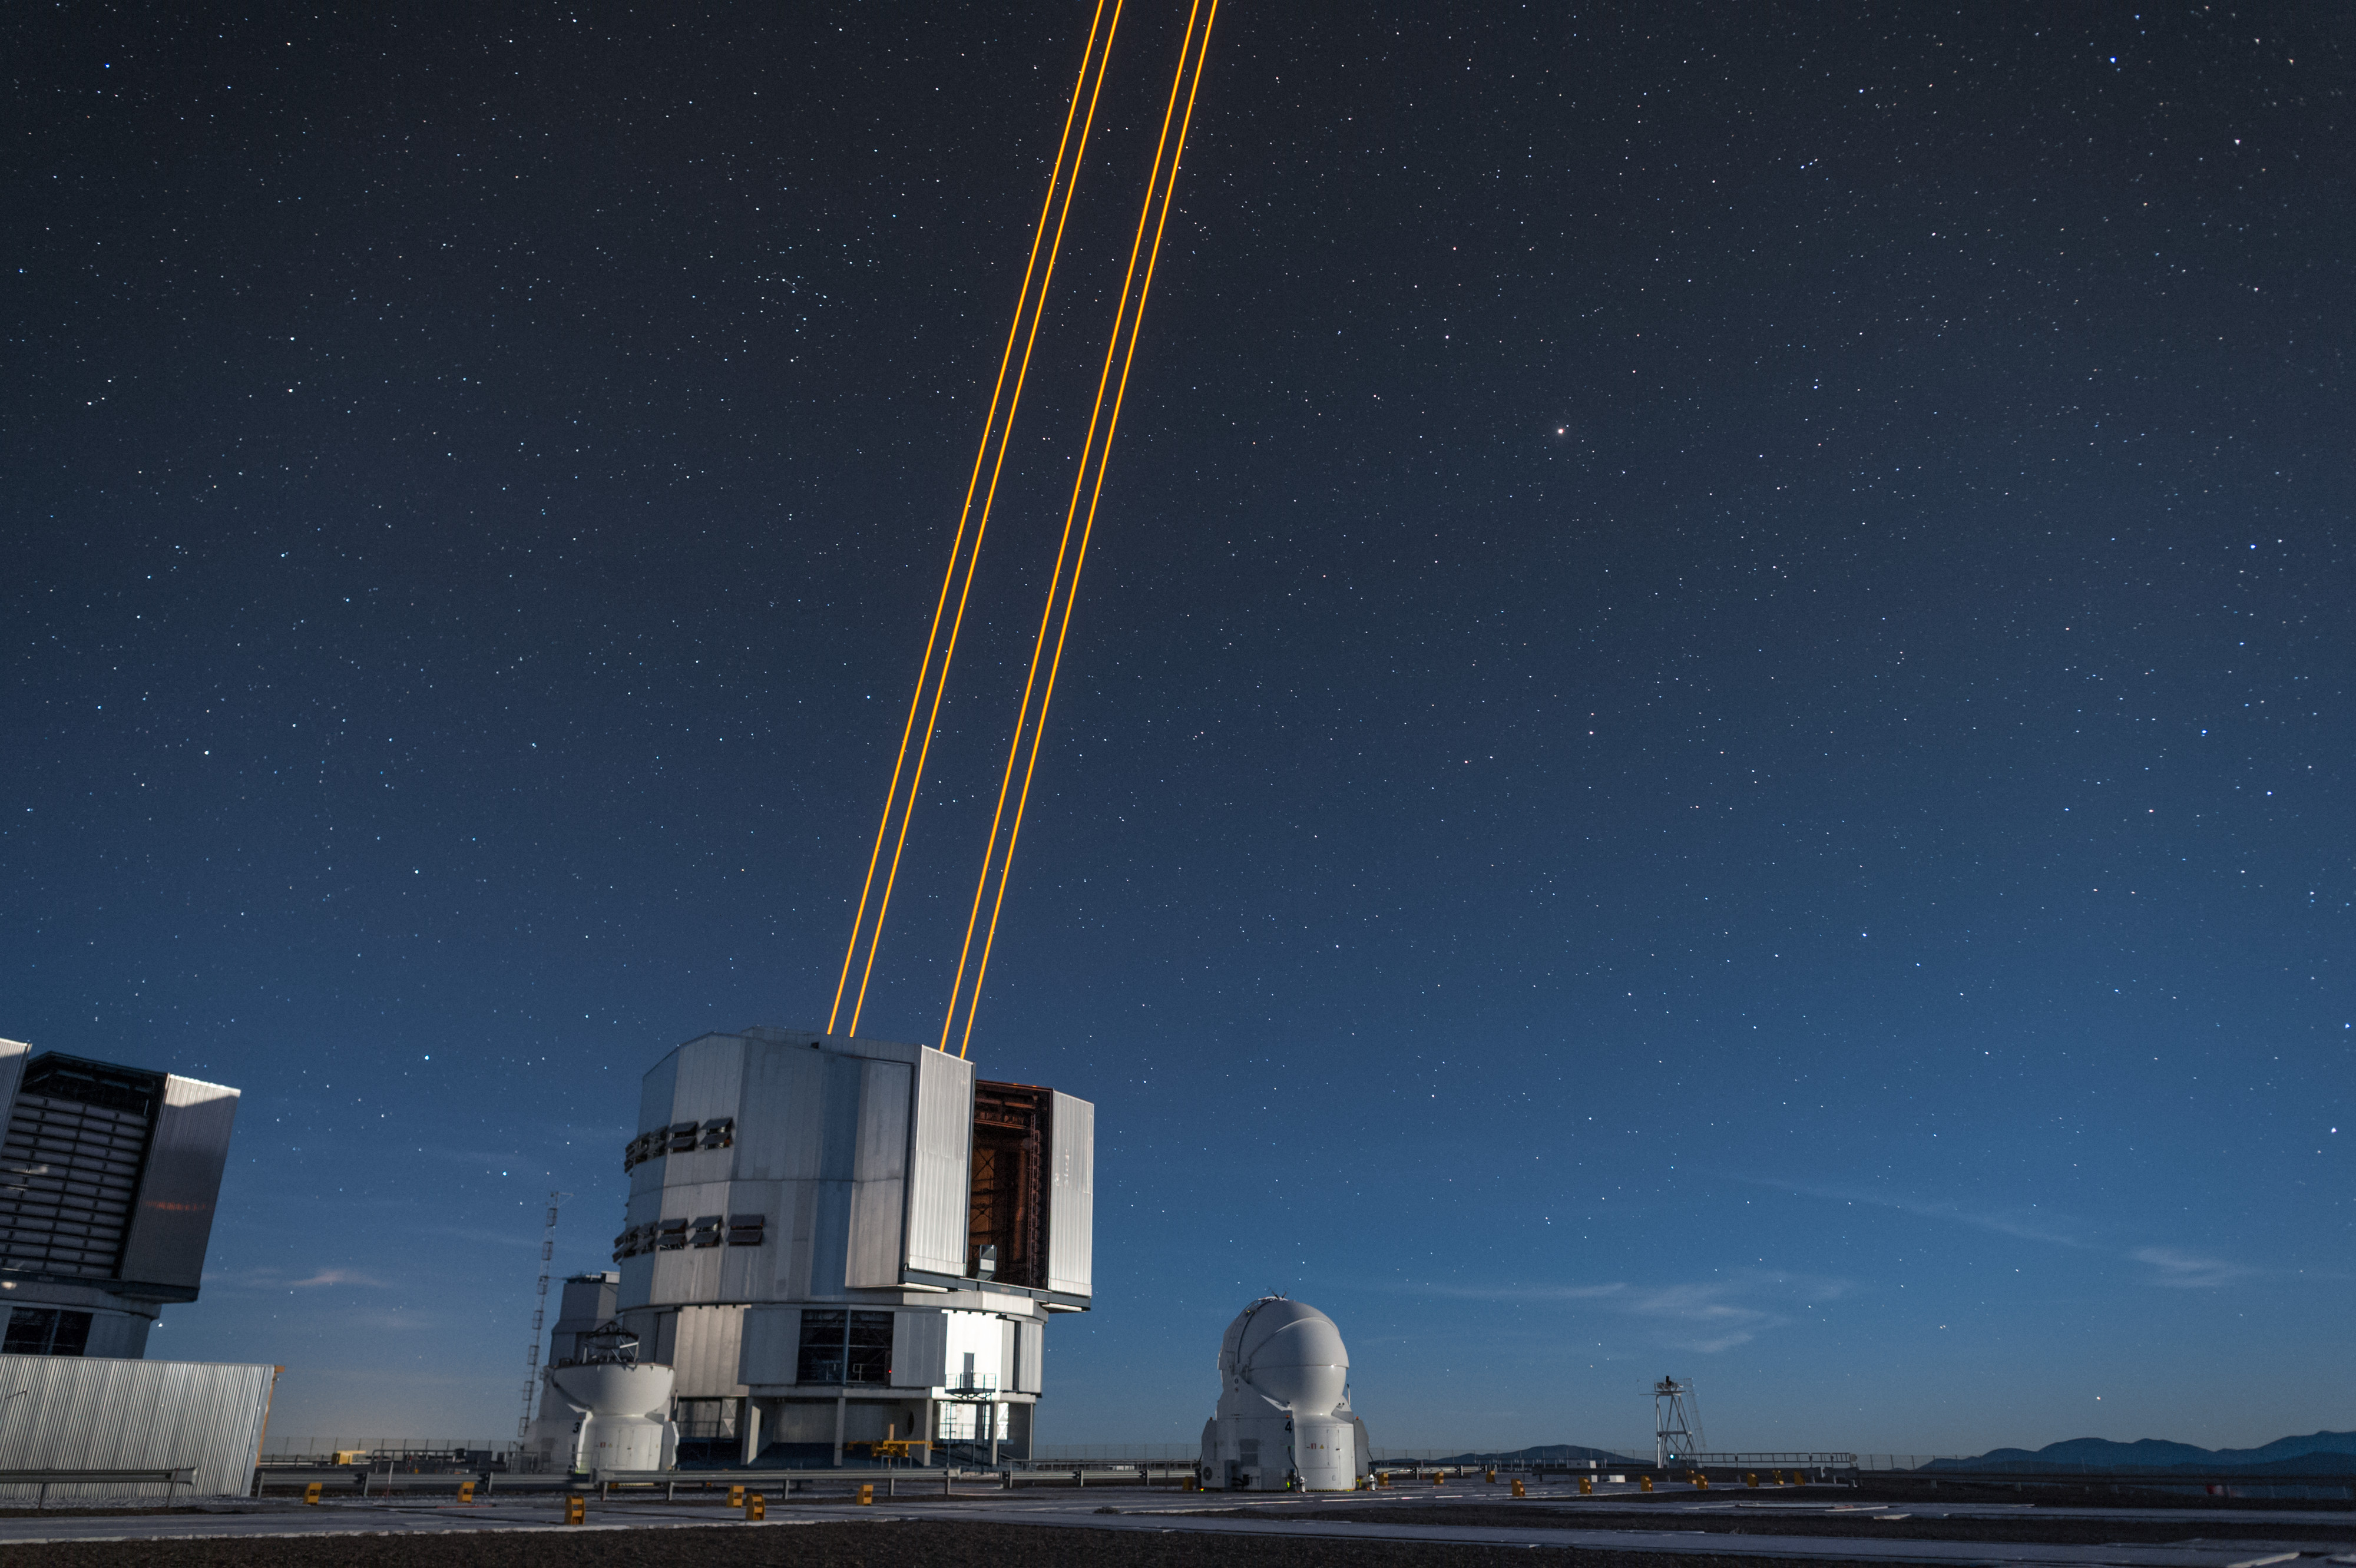
\includegraphics[width=0.7\textwidth]{adaptiv/images/Leitstern}
  \caption{Erzeugung eines Leitsterns (VLT der ESO Paranal Observatorium)
    \cite{eso:leitstern}}
  \label{fig:leitstern}
\end{figure}

\section{Kürzester Weg}
Wenn wir zwei Punkte im Raum betrachten und den kürzesten Weg zwischen ihnen suchen, so würden wir intuitiv die Punkte mit einer Geraden verbinden und diesen Weg als den kürzesten definieren. Wenn nun aber Licht den kürzesten Weg zwischen zwei Punkten sucht, wird nicht wie beim klassischen Weg die Strecke, sondern die Laufzeit, die das Licht benötigt, um den Punkt zu erreichen, minimiert. Weil zwischen den zwei Punkten eine Phasengrenze liegt, führt das dazu, dass der kürzeste Weg nicht mehr die direkteste Verbindung ist, sondern eine Streckte, die abhängig von Brechungsindex der beiden Phasen einem der möglichen Wege auf der Abbildung \ref{fig:weg} entspricht. Dieses Verhalten wird von Fermat's Prinzip beschrieben, welches besagt, dass der Weg des Lichtes zwischen zwei Punkten bezüglich der Laufzeit optimiert wird. Beim Suchen des kürzesten Weges befinden wir uns im Themengebiet der geometrischen Optik, Licht ist also nur ein Strahl. 

\begin{figure}
  \centering
  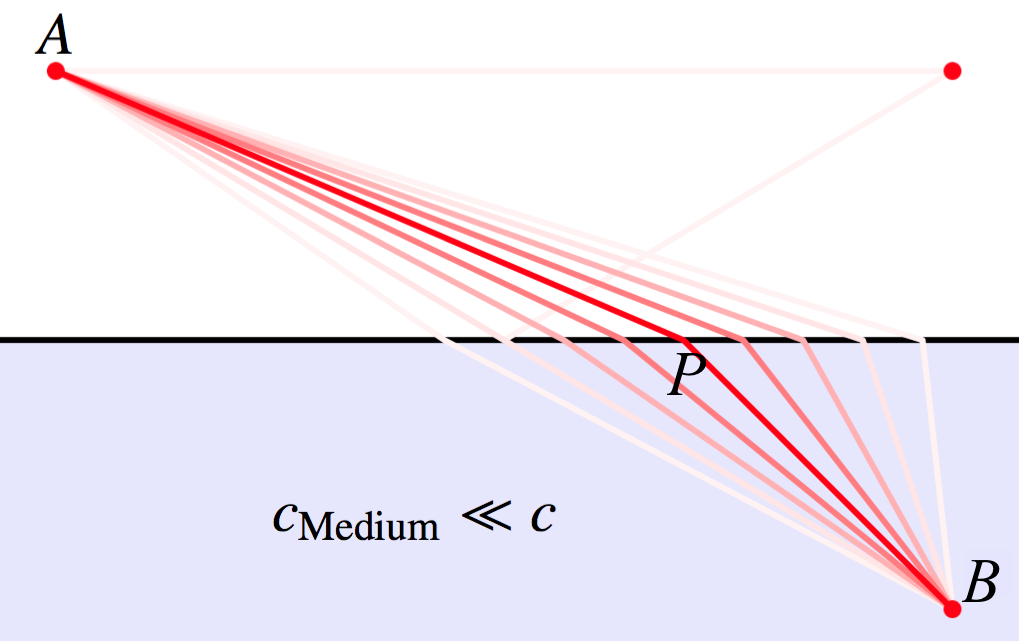
\includegraphics[width=0.6\textwidth]{adaptiv/images/Weg}
  \caption{Kürzester Weg zwischen zwei Punkten}
  \label{fig:weg}
\end{figure}
Welchen Weg nimmt aber Licht, wenn es wie in Abbildung \ref{fig:weg} von $A$ nach $B$ muss und dazwischen ein Übergang des Mediums stattfindet, wodurch das Licht nicht den intuitiv direkten Weg gehen kann? Nach dem Prinzip von Fermat soll die Zeit auf $\overline{AP}$ und $\overline{PB}$ minimal sein. Die Gleichung \eqref{bedmin} gibt die Bedingung an, mit welcher die Laufzeit vom Licht minimal ist:

\begin{equation}\label{bedmin}
\dfrac{\partial t}{\partial p_{x}}=0
\end{equation}
Um $t$ zu bestimmen, werden nun die Strecken $\overline{AP}$ und $\overline{PB}$ benötigt, die Punkte haben die folgenden Koordinaten $A = (0,a)$, $P=(p_{x},p_{y})$ und $B=(b,0)$. Die Gleichung \eqref{tbest} erklärt, wie aus Abbildung \ref{fig:weg} die jeweiligen Strecken bestimmt werden können. In einem weiteren Schritt wird die Gleichung \eqref{tbest} partiell nach $p_{x}$ abgeleitet und die Ableitung gleich Null gesetzt.

\begin{equation}\label{tbest}
t=\dfrac{s}{v}=\dfrac{\overline{AP}}{v_{1}}+\dfrac{\overline{PB}}{v_{2}}= 
\dfrac{\sqrt{(a-p_{y})^{2}+p_{x}^{2}}}{v_{1}}+ 
\dfrac{\sqrt{(b-p_{x})^{2}+p_{y}^{2}}}{v_{2}}
\end{equation}

\begin{equation}\label{partdiff}
\dfrac{\partial t}{\partial p_{x}}=
\dfrac{1}{v_{1}}\cdot \dfrac{1}{2 \sqrt{(a-p_{y})^{2}+p_{x}^{2}}}\cdot 2p_{x} +
\dfrac{1}{v_{2}}\cdot \dfrac{-1}{2 \sqrt{(b-p_{x})^{2}+p_{y}^{2}}}\cdot 2(b-p_{x})= 0
\end{equation}

\begin{equation}\label{glp}
\dfrac{n_{1}\cdot 2p_{x} }{\sqrt{(a-p_{y})^{2}+p_{x}^{2}}}+
\dfrac{-n_{2}\cdot 2(b-p_{x})}{\sqrt{(b-p_{x})^{2}+p_{y}^{2}}}= 0
\end{equation}

Die Geschwindigkeit $ v_{1}$ ist gleich $\frac{c}{n_{1}} $ und $ v_{2}$ ist gleich $\frac{c}{n_{2}}$, dabei ist $v_{i}$ die Lichtgeschwindigkeit im jeweiligen Medium. Wird nun in die Gleichung \eqref{partdiff} $ v_{1}$ und $ v_{2}$ eingesetzt und anschliessend mit $c$ multipliziert, erhält man die Gleichung \eqref{glp} aus welcher der Punkt $P$, respektive die Koordinate $p_{x}$ von $P$ bestimmt werden kann.
Abbildung \ref{fig:nullstelle} enthält eine grafische Darstellung der Ableitungen, dabei wird der Brechungsindex variiert und die Position des Punktes $P$ auf der Abbildung \ref{fig:weg} verändert seine Position in X-Richtung. Die  Punkte haben dabei die folgenden Koordinaten $A = (0,6)$, $P=(p_{x},3)$ und $B=(10,0)$. Für die Situation $n_{1}=n_{2}$ gibt es keinen Übergang, der Punkt $P$ hat die Koordinaten $(5,3)$ was genau dem direkten Weg entspricht. Mit den geeigneten Hilfsmitteln (Matlab) ist es möglich die Gleichung \eqref{glp} nach $p_{x}$ umzustellen, die Lösung ist aber unübersichtlich und sehr lang, die Abbildung \ref{fig:nullstelle} ist somit aussagekräftiger, der Schnittpunkt der X-Achse mit der Kurve entspricht dabei dem Wert $p_{x}$.
Damit ist der Strahlengang von $A$ nach $B$ via $P$ bestimmt. Dieser Weg ist minimal bezüglich der Laufzeit. \newline
Zur besseren Verständlichkeit noch eine kleiner Vergleich:

Gehen wir davon aus, dass kein Photon den Weg zurücklegen muss, sondern ein ausgesprochen intelligenter Hund. Er startet bei $A$ und muss bei $B$ einen Ball aus dem Wasser holen, die schwarze horizontale Linie auf der Abbildung \ref{fig:weg} stellt dabei das Ufer dar. Wenn der Hund den zuvor beschrieben Weg wählt, abhängig von seiner Geschwindigkeit an Land und im Wasser, ist er am schnellsten beim Ball, da er sich an Land schneller fortbewegen kann als im Wasser. Der Punkt $P$ ist somit der optimale Punkt für den Hund, um ins Wasser zu springen.

\begin{figure}
  \centering
  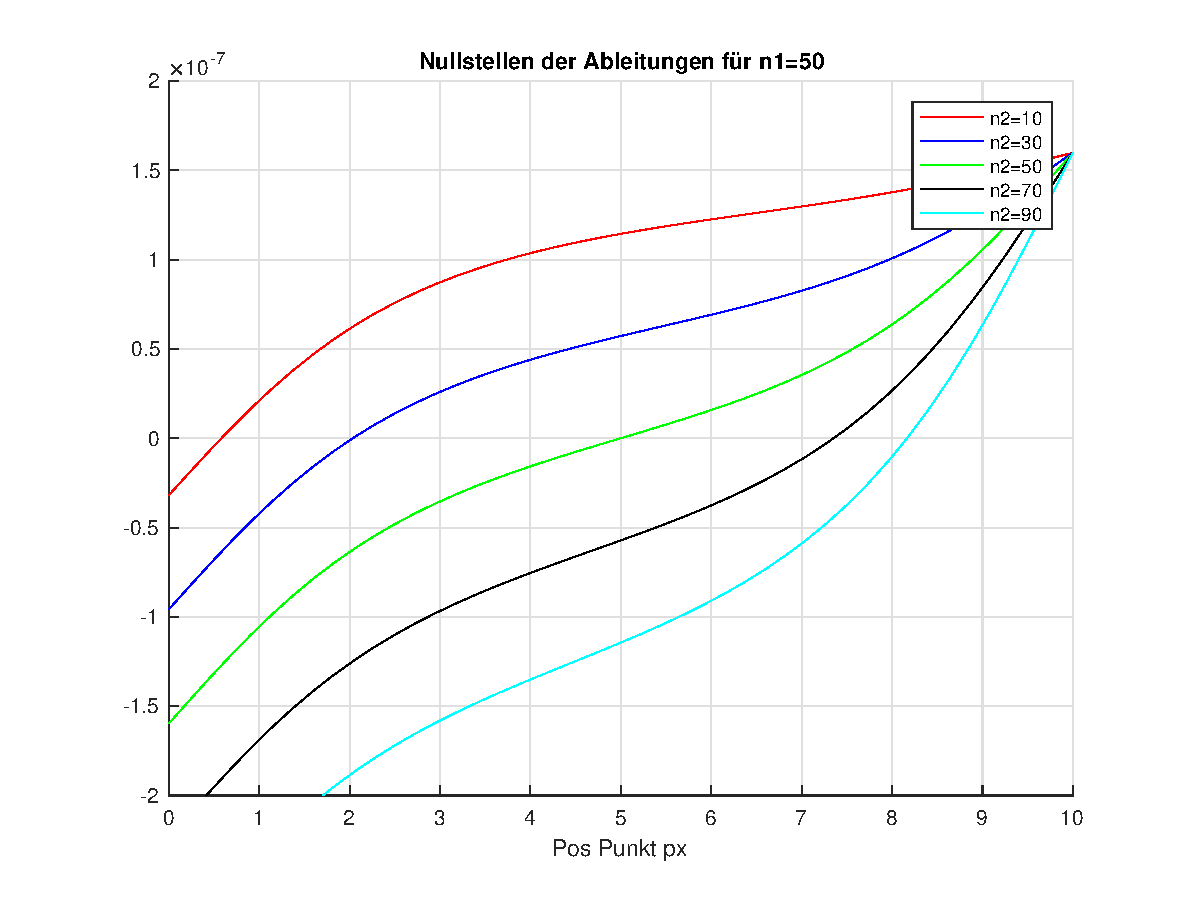
\includegraphics[width=0.9\textwidth]{adaptiv/images/Nullstellen}
  \caption{Nullstellen der Ableitung abhängig vom Brechungsindex}
  \label{fig:nullstelle}
\end{figure}

\subsection{Warum der kürzeste Weg}
Auf dem Weg von der Lichtquelle, in der Astronomie sind dies oft Sterne, Sternhaufen, Galaxien oder sogar ganze Cluster von Galaxien, trifft das Licht immer wieder auf Störeinflüsse. Störungen, die auf dem Weg durch das All entstehen, werden im nächsten Kapitel besprochen. Dieser Abschnitt handelt von Störungen, die in der Atmosphäre entstehen. Wenn mit einem Teleskop Sterne beobachtet werden, kann man immer von sehr gutem Wetter ausgehen und trotzdem die Atmosphäre vielschichtig aufgebaut und verursacht so Störungen. Das Licht sucht sich den schnellsten Weg durch die verschiedenen Schichten, dabei kommt es bei jedem Übergang zwischen zwei Schichten zu "Richtungsänderung" des Lichtes, wie in Abbildung \ref{fig:weg} dargestellt.

\section{Wellenfront}
Das Licht des Leitsterns, der mit dem Laser erzeugt wird, ist die Referenzlichtquelle, mit welcher man die Atmosphärenstörung messen kann. Die Atmosphärenstörung ist die Störung, die das Licht beim Passieren der jeweiligen Schicht erfährt. Dabei werden einige Näherungen gemacht, eine davon ist, dass auf der Hartmannplatte mit einer ebenen Wellenfront gerechnet wird, wie in Abbildung \ref{fig:hartmannplatte} zu erkennen ist. Der künstliche Leitstern ist aber eigentlich eine kugelförmige Quelle, warum also darf diese Näherung gemacht werden? Die Näherung ist möglich, da der Leitstern 90$km$ vom Sensor entfernt und die Krümmung der Wellenfront damit so gering ist, dass sie nur noch eine kleinen Einfluss hat und somit vernachlässigt werden kann, was die Berechnung vereinfacht. In Kapitel 4 wird das Thema der Krümmung behandelt, als kleine Anwendungsdemonstration wird im folgenden Abschnitt die Krümmung der kugelförmigen Welle berechnet.

\subsection{Krümmung der Wellenfront}
Die Wellenfront wird durch die Funktion \eqref{kugelfunktion} beschrieben. Davon soll nun die Krümmung berechnet werden, um den Fehler durch die Näherung bestimmen zu können. Korrekterweise müsste vor der Wurzel noch $\pm$ stehen, da sonst nur die obere Hälfte der Kugel betrachtet wird. Wir sind aber nur an der Krümmung der Kugel interessiert, die auf der ganzen Kugel gleich ist, weswegen  $\pm$ hier weggelassen wird.
\begin{equation}\label{kugelfunktion}
z=f(x,y)=\sqrt{r^{2}-x^{2}-y^{2})}
\end{equation}
Um die gausssche Krümmung zu berechnen, werden die ersten und zweiten partiellen Ableitungen und die Ableitung $ \frac{df}{dxdy}$ benötigt:

\begin{equation}\label{Ableitungen x}
f_{x}=\dfrac{\partial f(x,y)}{\partial x}= \dfrac{-x}{\sqrt{r^{2}-x^{2}-y^{2}}}
\end{equation}

\begin{equation}\label{Ableitungen xx}
f_{xx}=\dfrac{\partial f(x,y)}{\partial x^{2}}= \dfrac{- x^2}{(r^2 - x^2 - y^2)^{\frac{2}{3}}}+\dfrac{ - 1}{\sqrt{r^2 - x^2 - y^2}}
\end{equation}

\begin{equation}\label{Ableitungen y}
f_{y} =\dfrac{\partial f(x,y)}{\partial x}= \dfrac{-y}{\sqrt{r^{2}-x^{2}-y^{2}}}
\end{equation}

\begin{equation}\label{Ableitungen yy}
f_{yy}=\dfrac{\partial f(x,y)}{\partial y^{2}}= \dfrac{- x^2}{(r^2 - x^2 - y^2)^{\frac{2}{3}}}+\dfrac{ - 1}{\sqrt{r^2 - x^2 - y^2}}
\end{equation}

\begin{equation}\label{Ableitungen xy}
f_{xy}=\dfrac{\partial f(x,y)}{\partial x \partial y}=  \dfrac{-xy}{\sqrt{r^{2}-x^{2}-y^{2}}}
\end{equation}
Die Herleitung der Krümmung und die entsprechenden Beweise dazu sind in Kapitel 4 zu finden. Die gausssche Krümmung lässt sich berechnen, indem man die Gleichungen \eqref{Ableitungen x} bis \eqref{Ableitungen xy} in die Gleichung \eqref{gausskrümmung} einsetzt:  

\begin{equation}\label{gausskrümmung}
h = \dfrac{f_{xx} \cdot f_{yy} -f_{xy}^{2}}{(1+f_{x}^{2}+f_{y}^{2})^{2}} = \dfrac{1}{r^{2}} =\dfrac{1}{90000^{2}} = 1.234\cdot 10^{-10}
\end{equation}
Nach dem Einsetzen und Vereinfachen der Gleichung \eqref{gausskrümmung} erhält man den sehr einfachen Ausdruck $\frac{1}{r^{2}}$ für die Krümmung der Kugeloberfläche. Wie zu erwarten war, ist die Krümmung nicht von der Position auf der Kugel abhängig. 
Der daraus berechnete Wert ist mit $1.234\cdot 10^{-10}$ so klein, dass die Krümmung der Wellenfront vernachlässigt werden darf, ohne dass die Qualität der adaptiven Optik sich merklich verändert.

\section{Eikonalgleichung}
Beim kürzesten Weg haben wir gesehen, wie sich ein Lichtstrahl verhält, wenn er eine Phasengrenze überschreitet. Die Atmosphäre ist aber nicht aus einzelnen, scharf begrenzten Schichten aufgebaut, sie besteht aus stetigen Übergängen und ist zudem ständig in Bewegung. Der kürzeste Weg ist daher eine gute Veranschaulichung von einem einzelnen Übergang. Um aber den Weg eines Stahls durch die ganze Atmosphäre zu berechnen, muss eine Verallgemeinerung gemacht werden. Diese Verallgemeinerung führt schliesslich zur Eikonalgleichung \eqref{eikonal}, $n(r)^{2}$ ist dabei der Brechungsindex in Abhängigkeit von der Höhe: 

\begin{equation}\label{eikonal}
\left( \dfrac{\partial f}{\partial x}\right)^{2} + \left( \dfrac{\partial f}{\partial y}\right) ^{2} = n(r)^{2}
\end{equation}
Hier handelt  es sich um eine partielle nichtlineare Differentialgleichung, deren Lösung nicht ohne weiteres gefunden werden kann. Beim Lösen wird normalerweise eine nummerische Lösung gesucht, die mit dem Computer berechnet wird. Es gibt aber eine einfachere Lösung, die ohne Computer gefunden werden kann. Wir nehmen an, dass unser $n(r)$ konstant ist und setzen $f(x,y)=n\cdot\vec{e}\cdot\vec{x}= n(e_{1}x_{1}+e_{2}x_{2})$, wobei $\vec{e}$ der Normalenvektor der Wellenfront und $\vec{x}$ der Ortsvektor ist. Die partiellen Ableitungen davon sind die Gleichungen \eqref{eikdfx} und \eqref{eikdfy}:

\begin{equation}\label{eikdfx}
\dfrac{\partial f}{\partial x} = ne_{1}
\end{equation}
\begin{equation}\label{eikdfy}
\dfrac{\partial f}{\partial y} = ne_{2}
\end{equation}
Die Gleichungen \eqref{eikdfx} und \eqref{eikdfy} werden nun in die Gleichung \eqref{eikonal} eingesetzt, badei ist $(e_{1}^{2}+e_{2}^{2})=1$ die Länge des Einheitsvektors:

\begin{equation}\label{lösung_eik}
\left( \dfrac{\partial f}{\partial x}\right)^{2} + \left( \dfrac{\partial f}{\partial y}\right) ^{2} = \left( ne_{1}\right) ^{2}+\left( ne_{2}\right)^{2}=n^{2}(e_{1}^{2}+e_{2}^{2})=n^{2}
\end{equation}
Was bedeutet nun diese Lösung? Im Fall, dass $n(r)$ konstant ist. Die Erklärung dafür ist relativ einfach, es ist die selbe Situation wie beim kürzesten Weg, wenn beide Brechungsindizes gleich sind. Es kommt zu keiner Störung der Wellenfront, sie bleibt somit eine ebene Wellenfront und das Licht bewegt sich auf Strahlen, die Senkrecht zur Wellenfront verlaufen.

\subsection{Lösung durch Separation}
Eine weitere Möglichkeit zur Lösung zu kommen, ist der Separationsansatz. Die Idee dabei ist, dass die Funktion $f$ aus zwei einzelnen Funktionen aufgebaut ist, die nur von einer Variable abhängig sind, was beim Ableiten einen erheblichen Vorteil bringt. $f$ hat bei diesem Ansatz die Form der Gleichung \eqref{ansatzsep}, dieser Ansatz wird in die Gleichung \eqref{eikonal} eingesetzt:  

\begin{equation}\label{ansatzsep}
f(x,y)=X(x) + Y(y)
\end{equation}
Nach dem Einsetzen und Ableiten stellt man fest, dass auch für $n(r)$ eine Wahl getroffen werden muss, damit mit diesem Ansatz eine Lösung gefunden werden kann. In einem ersten Versuch wird $n(r)=y$ gesetzt, somit sind alle verbleibenden Funktionen nur von einer Variabel abhängig und es ist möglich, die Gleichung zu separieren. Dadurch erhalten wir die Gleichung \eqref{eikmitsansatz}:

\begin{equation}\label{eikmitsansatz}
X'(x)^{2}=y^{2}-Y'(y)^{2}
\end{equation}

\begin{equation}\label{sepx}
X'(x)^{2}=c \Rightarrow X'(x)=\sqrt{c}
\end{equation}

\begin{equation}\label{sepy}
Y'(y)^{2}=c-y^{2}  \Rightarrow Y'(y)=\sqrt{c-y^{2}}
\end{equation}
In der Gleichung \eqref{eikmitsansatz} wird einmal $x$ und einmal $y$ als konstant angenommen, dadurch erhalten wir zwei Gleichung, eine für $X'$ \eqref{sepx} und eine für $Y'$ \eqref{sepy}. Diese können einzeln gelöst und die Lösungen in den Ansatz \eqref{ansatzsep} eingesetzt werden. Für $X(x)$ erhalten wir so die Gleichung \eqref{X} und für $Y(y)$ die Gleichung \eqref{Y}, wobei die Lösungen durch eine Integration bestimmt werden müssen.

\begin{equation}\label{X}
X(x)=\sqrt{c}\cdot x
\end{equation}
\begin{equation}\label{Y}
Y(y)=\dfrac{1}{2}\left(y \sqrt{c-y^{2}}+c \cdot \arctan\left(  \dfrac{y}{\sqrt{c-y^{2}}}\right) \right) 
\end{equation}
Die beiden Funktionen können wieder mir einander addiert werden, womit eine weitere Lösung für $f(x,y)$  Gl\eqref{f(x,y)} gefunden wurde.

\begin{equation}\label{f(x,y)}
f(x,y)= \sqrt{c}\cdot x + \dfrac{1}{2}\left(y \sqrt{c-y^{2}}+c \cdot \arctan\left(  \dfrac{y}{\sqrt{c-y^{2}}}\right) \right) 
\end{equation}
In der Gleichung \eqref{f(x,y)} wird $f(x,y)$ als Parameter gesetzt, dadurch erhalten wir eine Implizite Gleichung, die sich darstellen lässt. 
Auf der Abbildung \ref{fig:plotwf1} ist die Ausbreitung der Wellenfront für $n(r)=y$ dargestellt, es ist gut zu erkennen, dass mit zunehmender Entfernung von der Quelle sich die Front immer weiter verformt. Bei der Abbildung \ref{fig:plotwf2} ist $n(r)= \sqrt{y}$, die Störung ist immer noch vorhanden, aber durch zunehmende Entfernung der Front von der Quelle, verändert sich die Front immer weniger, der Grund dafür ist die Charakteristik der Wurzelfunktion.
\begin{figure}
  \centering
  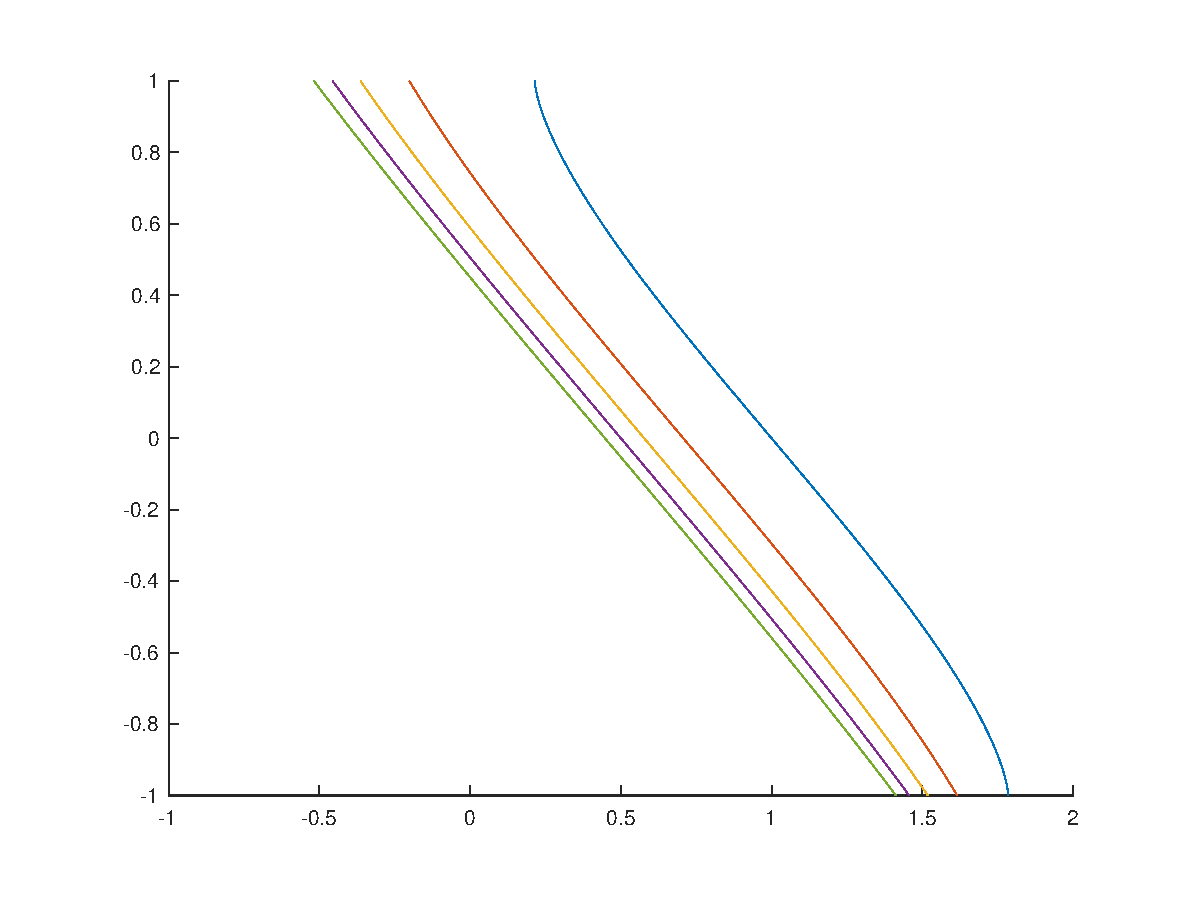
\includegraphics[width=0.8\textwidth]{adaptiv/images/plotwf1}
  \caption{Ausbreitung der Wellenfront in X-Richtung, für $n(r)=y$}
  \label{fig:plotwf1}
\end{figure}

\begin{figure}
  \centering
  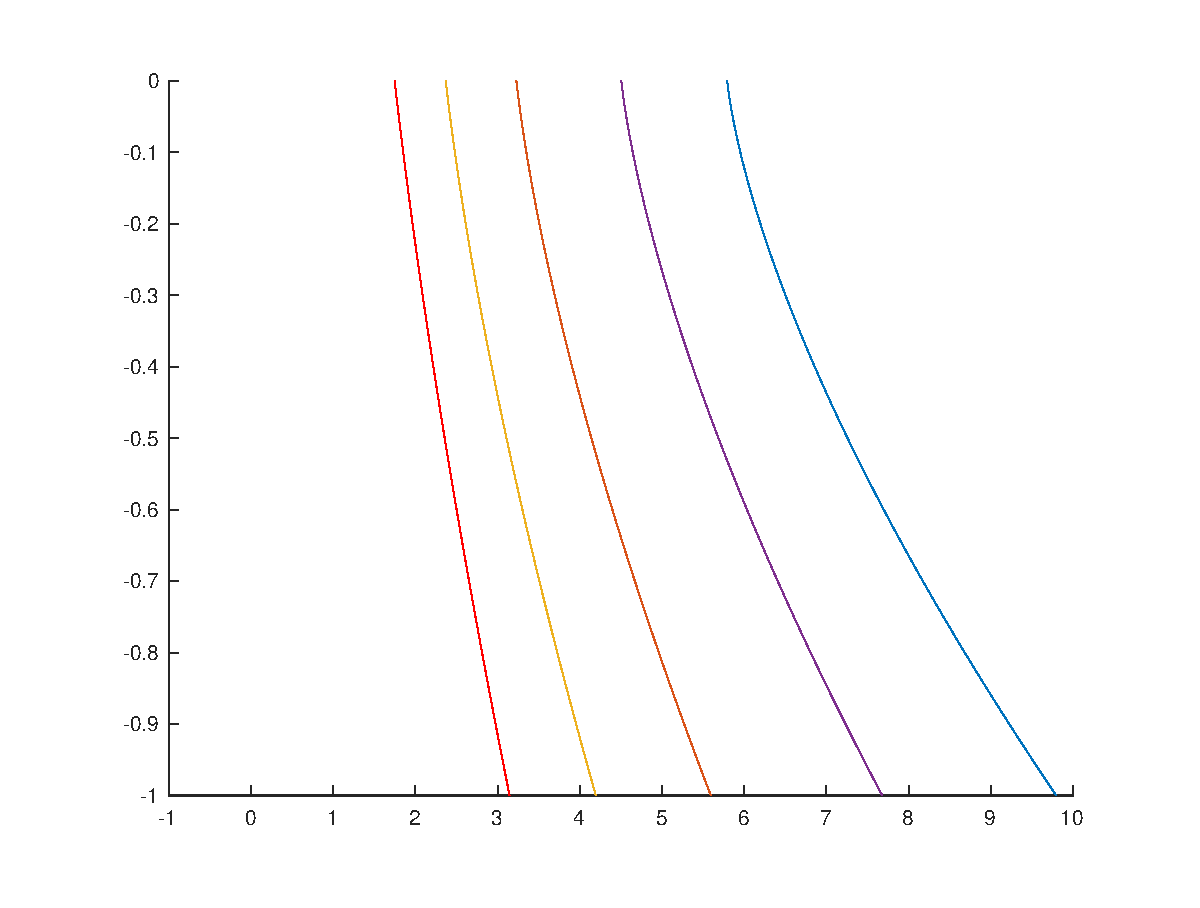
\includegraphics[width=0.8\textwidth]{adaptiv/images/plotwf2}
  \caption{Ausbreitung der Wellenfront in X-Richtung, für $n(r)=\sqrt{y}$}
  \label{fig:plotwf2}
\end{figure}

\printbibliography[heading=subbibliography]
\end{refsection}















